% 1.4.Solution.tex
%	Last update: 2019/10/03 F.Kanehori
%\newpage
\subsection{2oir3Im2bBWI9URv}
\label{subsec:Solution}

\noindent
\KLUDGE 前節で示した問題点への対処法について述べます。

\bigskip
\noindent
\bf{\KLUDGE ソースファイルの整合性}
\begin{narrow}[20pt]
	\SprLib \KLUDGE のソースツリーにあるプロジェクトディレクトリ
	(\tt{Base}, \tt{Collision}, ...)\KLUDGE を
	\KLUDGE 直接`\tt{add\_subdirectory}'\KLUDGE すれば問題ありません。
\end{narrow}

\medskip
\noindent
\bf{\KLUDGE ビルドの最適性(\KLUDGE 無駄なコンパイル)}
\begin{narrow}[20pt]
	\SprLib, \it{App1, App2\,}\KLUDGE などのすべてにおいて、
	\KLUDGE ライブラリのオブジェクトが生成される場所を共通化してしまうことで
	\KLUDGE この問題を回避することとします。
	\KLUDGE 具体的には、\SprLib \KLUDGE ソースツリーの中(\KLUDGE ビルドツリーの外)\KLUDGE に
	\KLUDGE オブジェクトの共通格納場所を作り、
	\SprLib \KLUDGE およびすべてのアプリケーションのオブジェクト格納領域が
	\KLUDGE そこを指すようにlink\KLUDGE を張ることとします。

\ifLwarp
	\begin{figure}[h]
	    \begin{center}
	    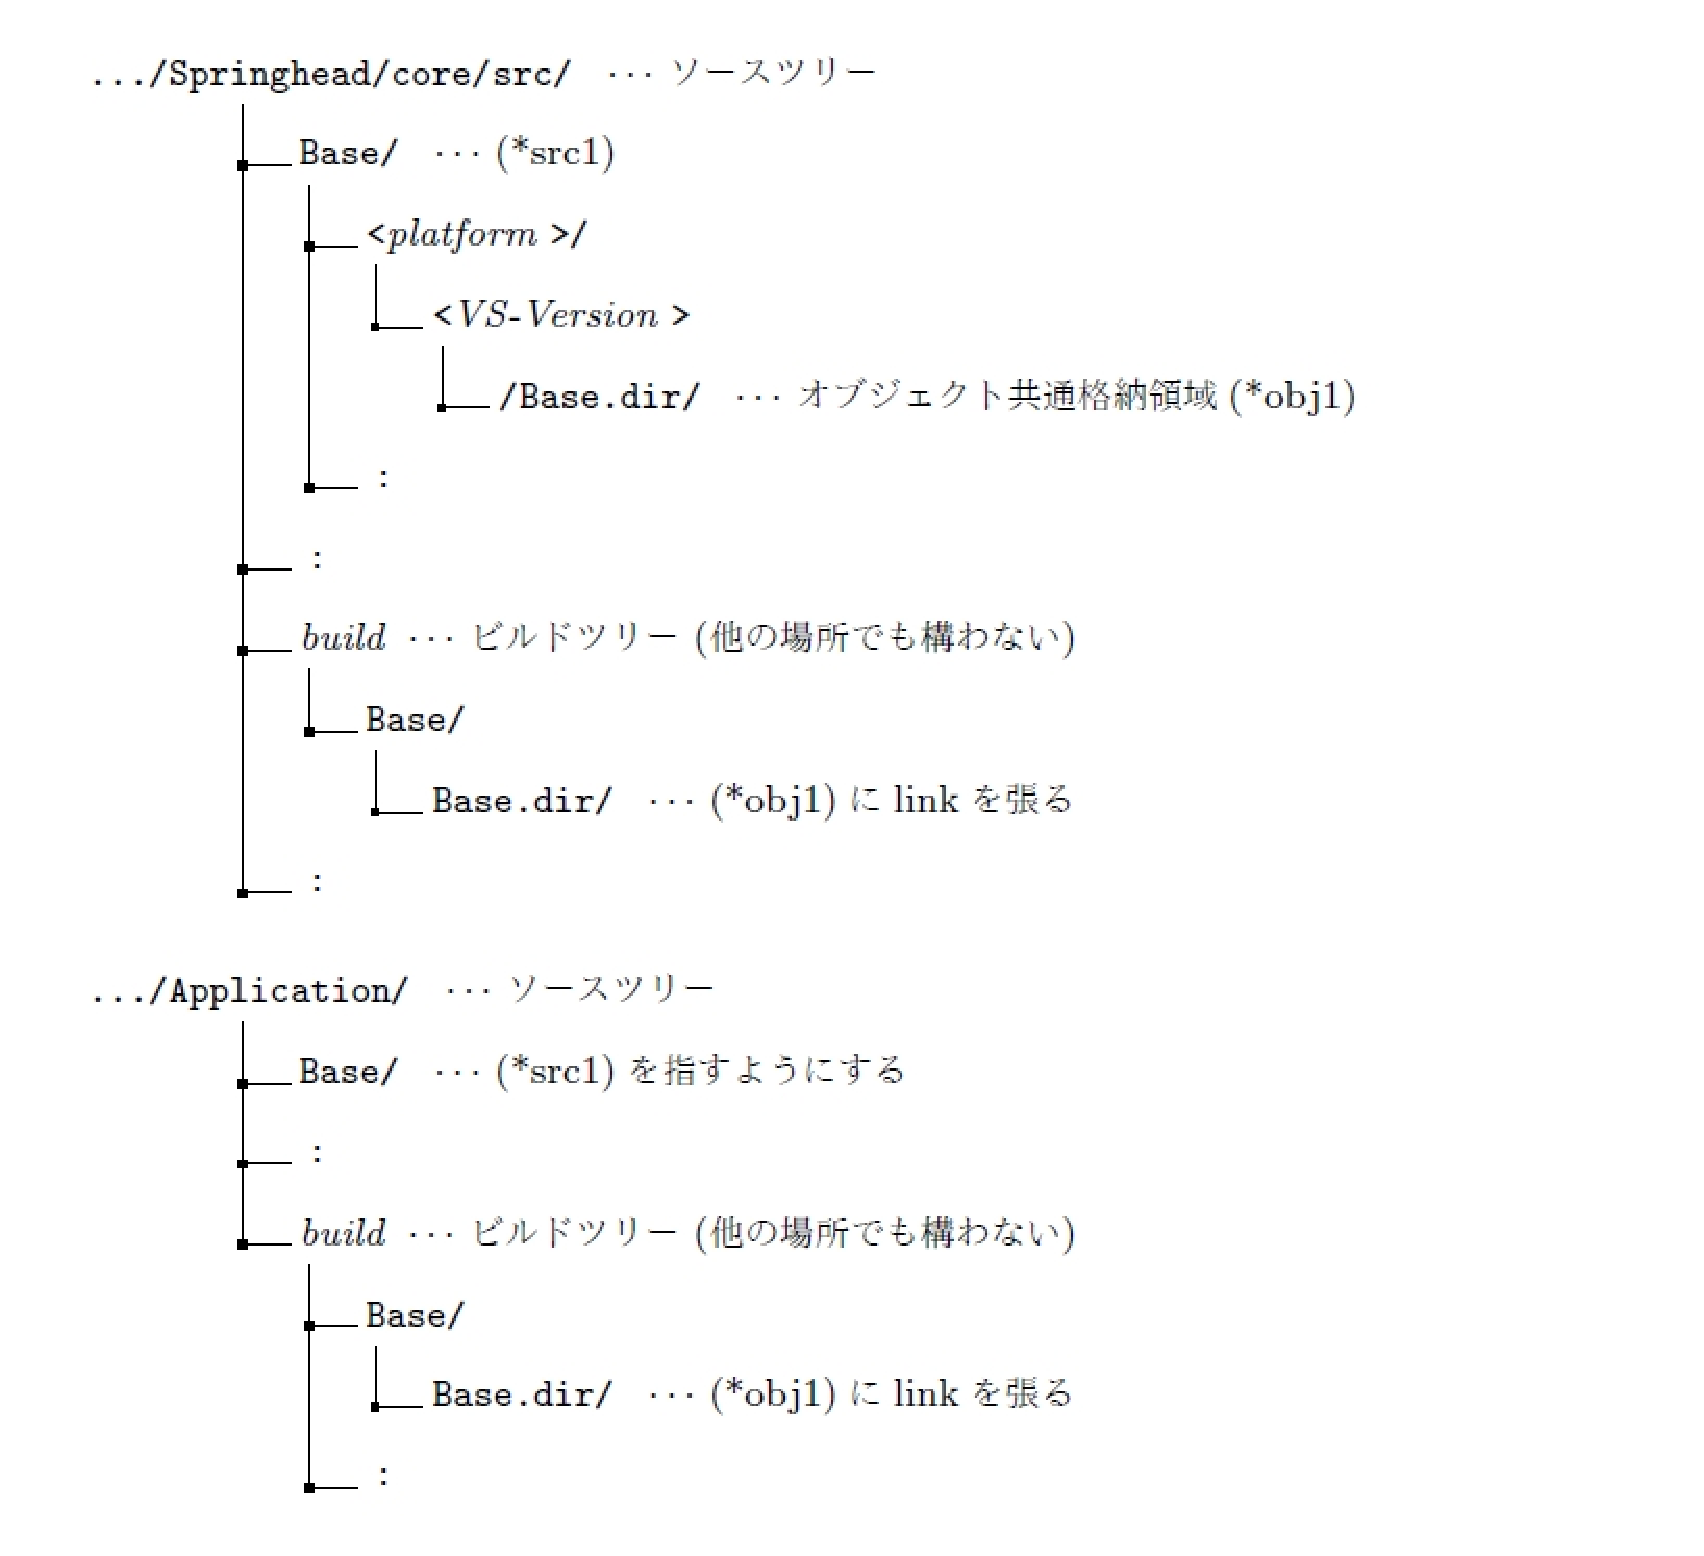
\includegraphics[width=.9\textwidth]{fig/ApproachToBuildOptimization.eps}
	    \end{center}
	    \caption{\KLUDGE ビルドの最適性への対処法}
	    \label{fig:ApproachToBuildOptimization}
	\end{figure}
\else
	\begin{figure}[h]
    	\begin{narrow}[40pt]\begin{minipage}{\textwidth}
		{\footnotesize{\dirtree{%
			.1 \hspace{-10mm}.../Springhead/core/src/ \Anno{\KLUDGE ソースツリー}.
			.2 Base/ \Anno{(*src1)}.
			.3 \textless \it{platform\,}\textgreater /.
			.4 \textless \it{VS-Version\,}\textgreater .
			.5 /Base.dir/ \Anno{\KLUDGE オブジェクト共通格納領域(*obj1)}.
			.3 \KLUDGE :.
			.2 \KLUDGE :.
			.2 \build \Anno{\KLUDGE ビルドツリー (\KLUDGE 他の場所でも構わない)}.
			.3 Base/.
			.4 Base.dir/ \Anno{(*obj1)\KLUDGE にlink\KLUDGE を張る}.
			.2 \KLUDGE :.
		}}}
		\medskip
    	\end{minipage}\end{narrow}
    	\begin{narrow}[40pt]\begin{minipage}{\textwidth}
		{\footnotesize{\dirtree{%
			.1 \hspace{-10mm}.../Application/ \Anno{\KLUDGE ソースツリー}.
			.2 Base/ \Anno{(*src1)\KLUDGE を指すようにする}.
			.2 \KLUDGE :.
			.2 \build \Anno{\KLUDGE ビルドツリー (\KLUDGE 他の場所でも構わない)}.
			.3 Base/.
			.4 Base.dir/ \Anno{(*obj1)\KLUDGE にlink\KLUDGE を張る}.
			.3 \KLUDGE :.
		}}}
		\medskip
  	\end{minipage}\end{narrow}
	\caption{\KLUDGE ビルドの最適性への対処法}
	\label{fig:ApproachToBuildOptimization}
	\end{figure}
\fi
	\indent
	\KLUDGE オブジェクトの共通格納領域を設定する作業は\SprLib \KLUDGE の\cmake\ (configure)\KLUDGE 時に、
	link\KLUDGE を張る作業はアプリケーションの\cmake\ (configure)\KLUDGE 時に行なうものとします。
\end{narrow}

\medskip
\noindent
\bf{\KLUDGE プロジェクトファイルの整合性}
\begin{narrow}[20pt]
	\KLUDGE ビルドの最適性の場合と同様、
	\KLUDGE プロジェクトファイルも共通化することでこの問題に対処します。
	\KLUDGE 具体的には、すべてのアプリケーションのプロジェクトファイルは、
	\SprLib \KLUDGE ビルドツリーにあるプロジェクトファイルを参照するlink\KLUDGE とします。

	\KLUDGE  ただしこれでは不完全で、\App{1}\KLUDGE で実施したプロジェクトファイルへの変更が
	\App{2}\KLUDGE に伝わりません。
	\KLUDGE このため\App{1}\KLUDGE でプロジェクトファイルを変更した場合には、
	\KLUDGE その変更を\SprLib \KLUDGE ビルドツリーにあるプロジェクトファイルに反映させるものとします。
	\KLUDGE つまり、\SprLib \KLUDGE のビルドツリーにあるプロジェクトファイルを
	\KLUDGE 常に最新の状態に保つということです。

	\KLUDGE  この作業はアプリケーションのビルド時に行なうものとします。
	\KLUDGE そのために、各アプリケーションのソリューションファイルに
	\KLUDGE 特別なターゲット`\tt{sync}'\KLUDGE を作成し、
	\KLUDGE このターゲットが毎回のビルドに先立って実行されるようにします。

\ifLwarp
	\begin{figure}[h]
	    \begin{center}
	    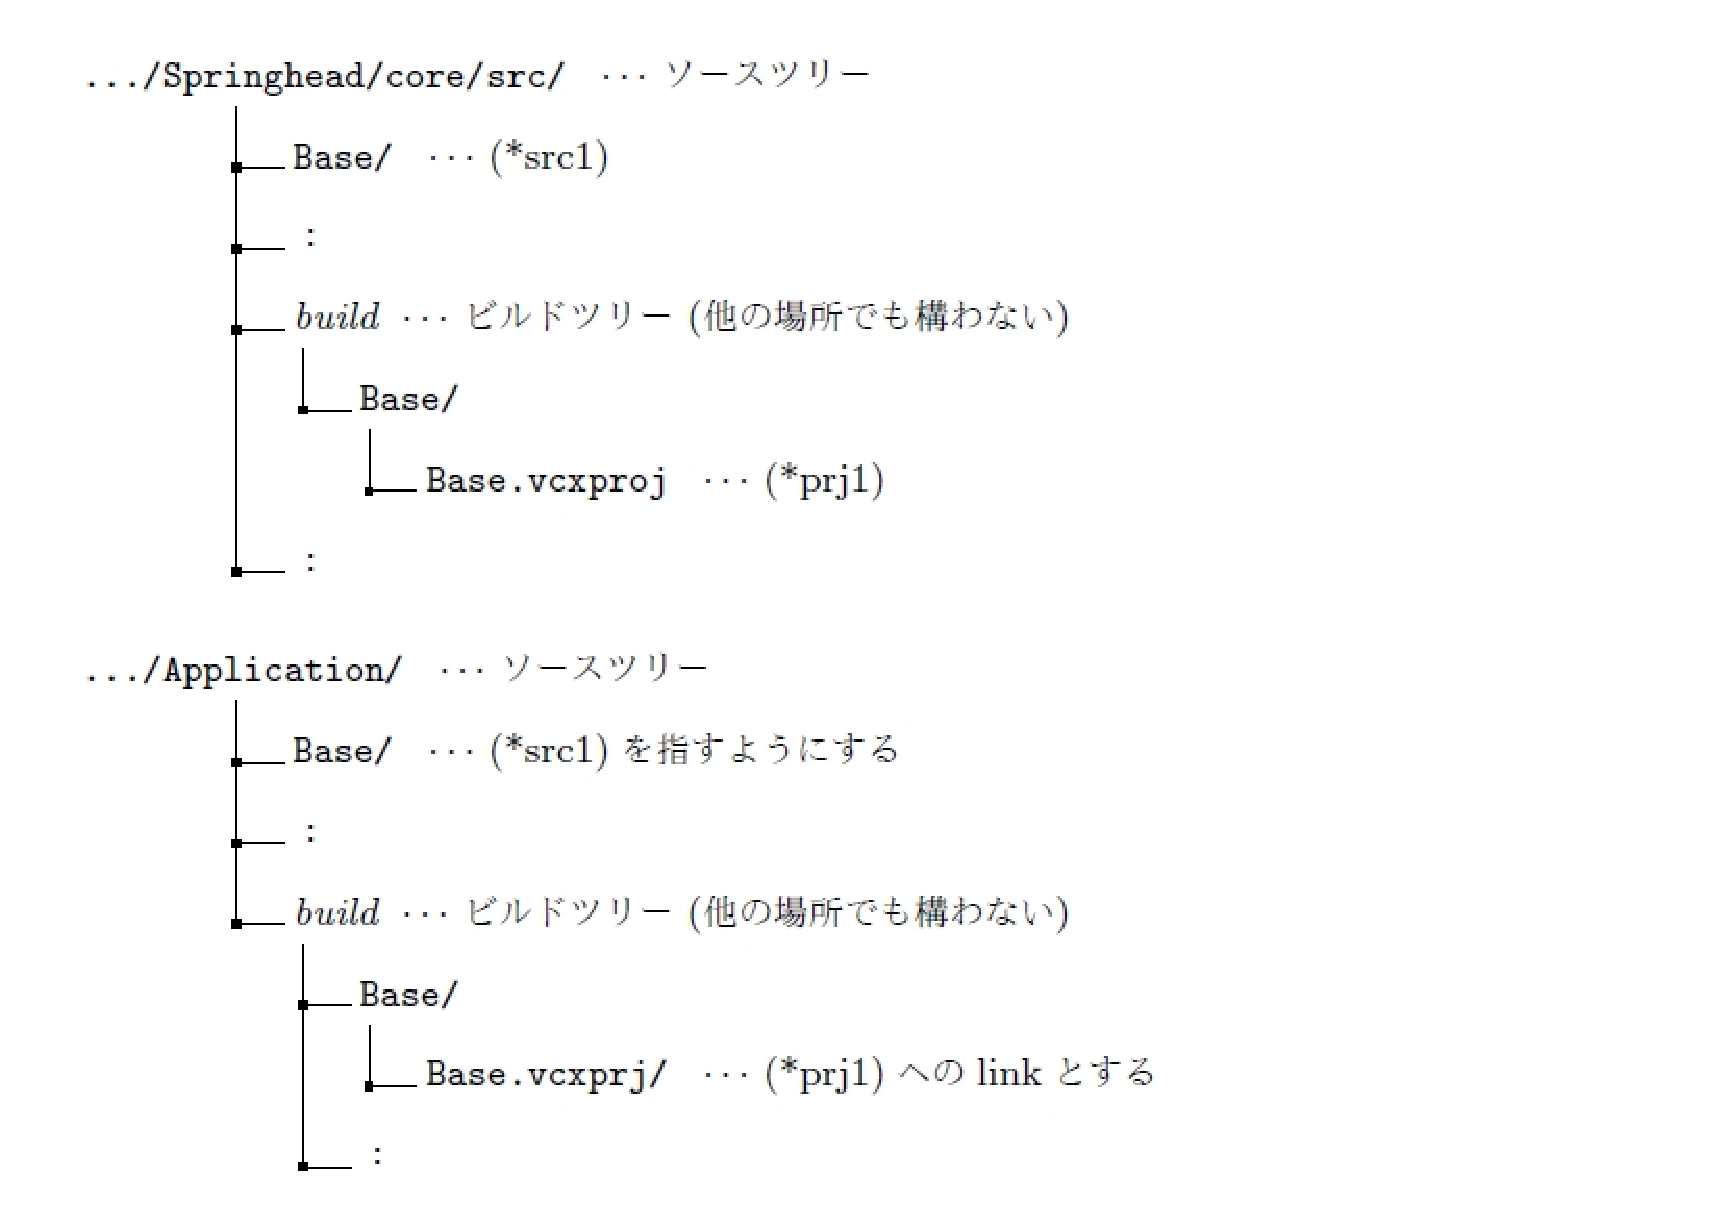
\includegraphics[width=.9\textwidth]{fig/ApproachToProjfileOptimization.eps}
	    \end{center}
	    \caption{\KLUDGE プロジェクトファイルの最適性への対処法}
	    \label{fig:ApproachToProjfileOptimization}
	\end{figure}
\else
	\begin{figure}[h]
    	\begin{narrow}[40pt]\begin{minipage}{\textwidth}
		{\footnotesize{\dirtree{%
			.1 \hspace{-10mm}.../Springhead/core/src/ \Anno{\KLUDGE ソースツリー}.
			.2 Base/ \Anno{(*src1)}.
			.2 \KLUDGE :.
			.2 \build \Anno{\KLUDGE ビルドツリー (\KLUDGE 他の場所でも構わない)}.
			.3 Base/.
			.4 Base.vcxproj \Anno{(*prj1)}.
			.2 \KLUDGE :.
		}}}
		\medskip
    	\end{minipage}\end{narrow}
    	\begin{narrow}[40pt]\begin{minipage}{\textwidth}
		{\footnotesize{\dirtree{%
			.1 \hspace{-10mm}.../Application/ \Anno{\KLUDGE ソースツリー}.
			.2 Base/ \Anno{(*src1)\KLUDGE を指すようにする}.
			.2 \KLUDGE :.
			.2 \build \Anno{\KLUDGE ビルドツリー (\KLUDGE 他の場所でも構わない)}.
			.3 Base/.
			.4 Base.vcxprj/ \Anno{(*prj1)\KLUDGE へのlink\KLUDGE とする}.
			.3 \KLUDGE :.
		}}}
		\medskip
  	\end{minipage}\end{narrow}
	\caption{\KLUDGE プロジェクトファイルの最適性への対処法}
	\label{fig:ApproachToProjfileOptimization}
	\end{figure}
\fi
	\indent
	
\end{narrow}

% end: 1.4.Solution.tex
